\documentclass[11pt,a4paper]{book}
\usepackage{listings,textcomp,graphicx,float,verbatim,extsizes}
\usepackage{amsmath,amssymb,mathrsfs}
\usepackage{sectsty}
\usepackage[left=3.2cm, right=3.2cm, top=3cm, bottom=4cm]{geometry}

%setup links
\usepackage{hyperref}
\hypersetup{
    colorlinks,
    citecolor=black,
    filecolor=black,
    linkcolor=black,
    urlcolor=black
}
%\hypersetup{linktocpage} to only make page number in toc clickable

\usepackage{fancyhdr}

\pagestyle{fancy}
\setlength{\headheight}{15.2pt}
\fancyhead[LE,RO]{\slshape \rightmark}
\fancyhead[LO,RE]{\slshape \leftmark}
\fancyfoot[C]{\thepage}
\begin{comment}

\lhead{}
\chead{}
\rhead{}
\lfoot{}
\cfoot{\thepage}
\rfoot{}
\end{comment}

\makeatletter
\renewcommand{\@makechapterhead}[1]{%
\vspace*{50 pt}%
{\setlength{\parindent}{0pt} \raggedright \normalfont
\bfseries\Huge
\ifnum \value{secnumdepth}>1
   \if@mainmatter\thechapter.\ \fi%
\fi
#1\par\nobreak\vspace{40 pt}}}
\makeatother

\title{Individual Project\\Expression Transfer}
\author{Martin Papanek (mp5309)}
\date{}


\begin{document}

\maketitle

\begin{center}
\LARGE \textbf{Abstract}
\end{center}

\newpage

\begin{center}
\LARGE \textbf{Acknowledgements}
\end{center}


\newpage

\tableofcontents
\listoftables

\chapter{Introduction}
\section{Motivation}
Allowing computers to understand the world around them is one of the most
intriguing goals of computer science. In order to aid humans in day-to-day
tasks,the ideal computer should perceive his surroundings, correctly identify the objects and beings around him and act based
on this information. Achieving this level of sophisticated, environment aware
behaviour is the focus of popular computer science fields such as machine
learning, computer vision and logic.

The problem of understanding the surrounding world can be broken down into a
number of sub-problems. First the machine must obtain and process the information on
its sensors. Then it has to utilize the data gleaned from its sensors to find
objects in the image. Finally, the machine has to obtain contextual information
from the configuration of these objects. Possessing this contextual information can be seen
as equivalent to understanding the scene. The computer uses the contextual
information to understand what state the environment is in and can then act based on
simple if-then rules.

For humans, all of the aforementioned sub-problems seem simple. However, programming
machines to do the same is quite difficult. Computers often do
possess better sensors than most humans and thus are readily able to obtain data
from sensors. Yet, they are sorely lacking when it comes to locating objects
in this sensory input and correctly assessing the properties and configuration
of these objects. While it is possible to locate circles and lines, joining
these to locate a face or a tree can only be done if the machine knows what a
face or a tree should look like. To instruct machines about the properties of
the various objects, which could potentially be present in the surroundings, we
use \textit{models}. A model describes the expected structure of the object.
This, in turn, allows the machine to explain aspects of its sensory input as the
occurence of that object. Finding objects by means of locating an instance of a
model in the input is called \textit{model-based tracking}.

Certain objects may also change their shape or
appearance. For example a face may transition from a closed eyed state to an
open eyed state. An even better example is the body of a human, which is also
highly dynamic. These deformable objects are often of special interest to us in
our everyday life. A machine should therefore be able to recognize an arbitrarily deformed
object and also correctly identify the shape or appearence of this dynamic
object. The challenge thus lies in constructing an appropriate \textit{deformable
model}. 

Furthermore, the computer has to be able to find an instance of this
model in its surroundings if and only if this object is present. This task is
known as \textit{model extraction}. When extracting deformable models, it is
necessary to also estimate what state the model is in. This means we have to not
only locate the object but also estimate the values of parameters which govern how this
object changes.

Hence, in this paper we are interested in describing convenient dynamical shape
and appearence models and effective algorithms for locating these models. For our
sensory snapshots, we will focus exclusively on images. Since we will be dealing
with images we will investigate motion tracking and feature detection
algorithms. These are necessary to obtain cues from our input image which allow
us to locate the model in the image.

 The area where deformable models
are applicable is quite large. This paper will focus on one very interesting application of dynamical
models and model extraction which is
\textit{expression transfer}.  The purpose of expression transfer is to capture the expressions and visemes
(speech related mouth articulations) from a video recording of one individual and
generate a video of another individual mimicking these
expressions and visemes. The alternative to transferring these expressions would
be to construct a physical model of the face and simulate the observed
expressions and visemes using the model. However, transferring the dynamics of a subjects face to that of another enables us to
create very realistic animations without much difficulty. On the other hand, it
is quite difficult to generate realistic expressions by setting the appropriate
parameters of a physical model simply because of the complexity of the physics
behind the movement that is responsible for expressions.

\section{Contributions}

\section{Report Overview}

\newpage

\chapter{Background}
Using models to characterise a deformable object and locate it in an image remains
a very fundamental challenge of computer vision and graphics. In this chapter we
will examine various model extraction techniques. Likewise, we will discuss
computer vision algorithms that will allow us to locate the parts that make up
our objects and observe how the objects change between several images.
\section{Model-based object recognition}
The goal of model-based object recognition is to fit an instance of a model to
an the appropriate object in the image. The problem of fitting the model to the
image is in essence an optimization problem. In order to fit the model we need to
correctly adjust parameters that control the model. In addition to determining
the intrinsic parameters of the model it is necessary to also find how the
object is rotated, moved and scaled. The parameters which determine the
orientation are called \textit{pose parameters}. 

\subsection{Shape Model}
A \textit{shape model} describes the boundaries of an object. figure 111 For example a
shape model of a face which denotes the location and measures of the defining
contours of a face. To locate an object in an image the shape model must be able to
account for the following
\begin{itemize}
\item variations of shape due to deformations of the object
\item arbitrary scaling of the object
\item arbitrary rotations of the object
\item some measure of gaussian input noise tolerance
\end{itemize}


   

\subsection{PCA and Eigenfaces}
In 1991, Turk and Pentland \cite{eigenfaces91} pioneered a face recognition approach
based on the mathematical
technique called principal component analysis (PCA). Their face recognition
scheme uses a data set of images to learn what they call
\textit{eigenfaces}. Expressed in mathematical terms - the eigenfaces are principal components of the 2D image
space. They represent the vectors of the 2D data set that are responsible for any
significant variation. 
As such these vectors are the eigenvectors of the covariance matrix of the face
images. To obtain the eigenfaces it is necessary to compute the SVD decomposition of this
covariance matrix. Any individual face from the training data set can then be
exactly represented as a linear combination all the eigenfaces.

\begin{figure}[H]
\centering
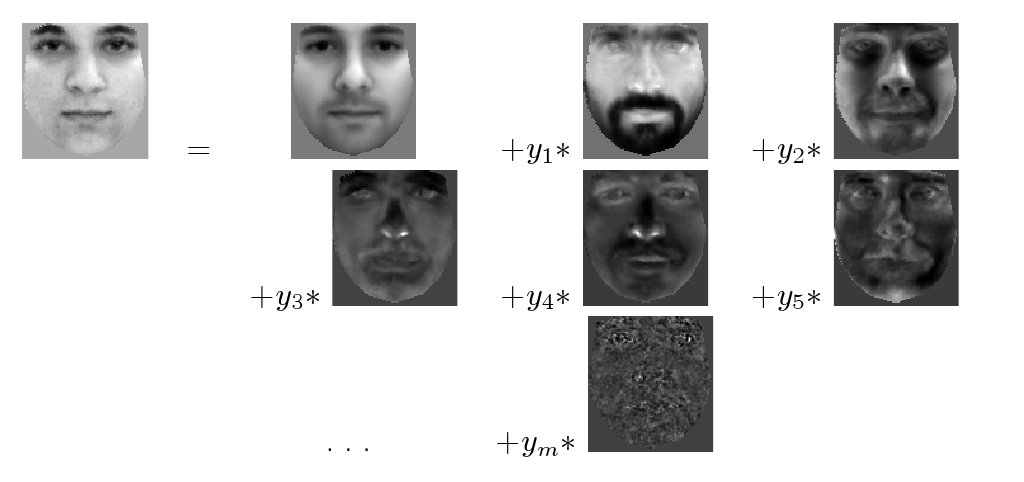
\includegraphics[scale=0.5]{images/eigenfaces_comb_from_nn_vienna.png}
\caption{ Using the eigenfaces we can represent an image as a linear combination of the
  eigenfaces. Taken from \cite{vienna} }
\label{gr:eigenfaces}
\end{figure}

The weight of each eigenface in the linear combination is computed from the
projection of the face image onto this eigenface. To recognize a face we
 first calculate these weights. Then we calculate the euclidean distance of the vector
of weights to the weights of faces from our training data set. The face from
the data set with weights which are closest to the new image's weights is chosen
as a match.

In an image of 256 by 256 we have a 65,536 dimensional vector that
represents the face image. This means we would require 65,536 eigenfaces to be
able to exactly represent every face. However, images of faces are very similar
in their configuration which means that the underlying principal subspace of
faces has a lower dimension than 65,536. Once the eigenfaces which span this
principal subspace are found we can
effectively encode a 65,536 dimensional vector using a vector of much smaller
dimensions. 

The main advantage of the eigenfaces is that we can approximate a face very well
by a linear combination of only the eigenfaces that account for the largest
variance. The set of $M$ eigenfaces that represent the $M$ largest variances is called
the \textit{face space}.

The drawback of a PCA based model is that the recognition rate drops significantly once
independent sources of variation are introduced. Turk and
Pentland noted that the eigenfaces approach has issues with variations in lighting,
head size, head orientation or faces exhibiting expressions \cite{eigenfaces91}. Likewise, when
faces are partially occluded in images it causes difficulties to the technique. 

The eigenfaces approach is based heavily information and coding theory
\cite{eigenfaces91}. With the PCA it is possible to encapsulate a face image
using low dimensional vector. As such PCA and eigenfaces are often used to
reduce dimensionality in more sophisticated modelling approaches.

\section{Model-based tracking}


\bibliographystyle{plain}
\bibliography{references}

\end{document}
